\section{实验八\ 文件系统}

\subsection{实验目的}

\begin{enumerate}
    \item 了解 MINIX 文件系统的发展。
    \item 掌握虚拟文件系统的概念。
    \item 掌握高速缓冲区相关的数据结构与算法。
    \item 了解内核对竞争条件的处理。
\end{enumerate}

\subsection{文件系统布局概览}

Linux 0.11 内核的文件系统参照了 MINIX 文件系统 1.0 版。

MINIX 文件系统与标准 UNIX 的文件系统基本相同,由 6 个部分组成。

\begin{figure}[htbp]
    \centering
    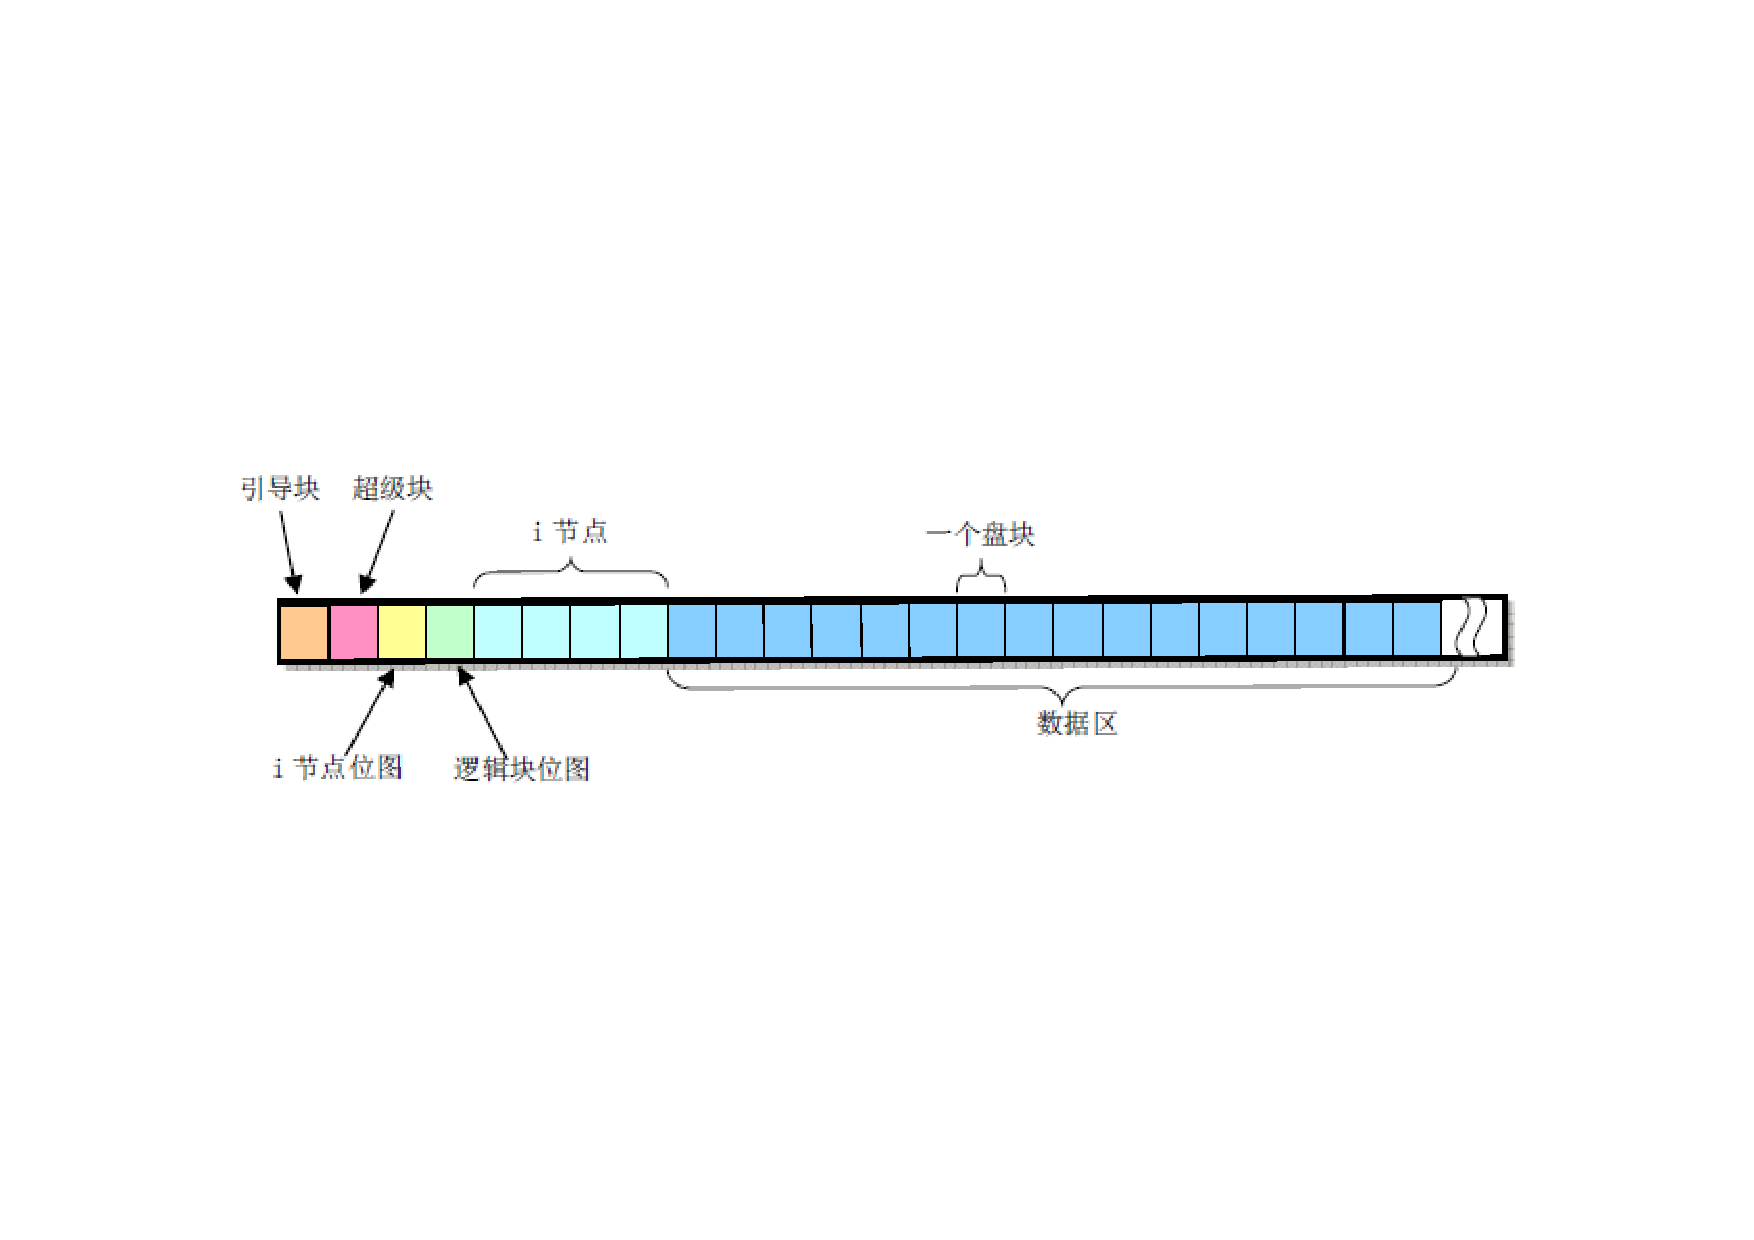
\includegraphics[width=\textwidth]{img/建有MINIX文件系统的一个360KB软盘中文件系统各部分的布局示意图.pdf}
    \caption{建有 MINIX 文件系统的一个 360KB 软盘中文件系统各部分的布局示意图}
    \label{fig:建有MINIX文件系统的一个360KB软盘中文件系统各部分的布局示意图}
\end{figure}

\textbf{引导块}是计算机加电启动时可由 ROM BIOS 自动读入的执行代码和数据。但并非所有盘都用作引导设备,对于不用于引导的盘片,这一盘块中可以不含代码。但任何盘片必须含有引导块,以保持 MINIX 文件系统格式的统一。

\textbf{超级块}用于存放盘设备上文件系统结构的信息,并说明各部分的大小。

\textbf{i 节点位图}用于说明 i 节点是否被使用,每个比特位代表一个i节点。

\textbf{逻辑块位图}用于描述盘上的每个数据盘块的使用情况,每个比特位代表盘上数据区中的一个数据盘块。

盘上的 i 节点部分存放着文件系统中文件(或目录)的索引节点,每个文件(或目录)都有一个 i 节点。每个 i 节点结构中存放着对应文件的相关信息。

文件中的数据是放在磁盘块的数据区中的,而一个文件名则通过对应的 i 节点与这些数据磁盘块相联系。

\subsubsection{文件的分类}

类 UNIX 操作系统中的文件通常分类 6 类。在 Linux 的 Shell 下执行 “ls -l” 命令,可从文件状态信息中查看文件的类型。

\begin{enumerate}
    \item \textbf{正规文件}是一类文件系统对其不作解释的文件,包含任意长度的字节流。源程序文件、二进制执行文件、文档以及脚本文件都是正规文件。
    \item \textbf{目录}(‘d’)在 UNIX 文件系统中也是一种文件,但文件系统管理会对其内容进行解释,使人们看到有哪些文件包含在一个目录中,以及它们是如何组织在一起构成一个分层次的文件系统的。
    \item \textbf{符号连接}(‘s’)用于使用一个不同的文件名来引用另一个文件。符号连接可以跨越文件系统,把一个文件名连接到另一个文件系统中的一个文件上。
    \item \textbf{命名管道}(’p’)文件是系统创建有名管道时建立的文件。可用于无关进程之间的通信。
    \item \textbf{字符设备}(’c’)文件用于访问字符设备,例如 tty 终端、内存设备以及网络设备。
    \item \textbf{块设备}(’b’)文件用于访问像硬盘、软盘等设备。
\end{enumerate}

\subsubsection{高速缓存}

CPU 中的高速缓存(cache)是用于减少处理器访问内存所需平均时间的部件,其容量远小于内存,但速度却可以接近处理器频率。

Linux 内核实现高速缓存的程序是 Linux-0.11/fs/buffer.c。文件系统中其他程序通过指定需要访问的设备号和数据逻辑块号来调用它的块读写函数。

\subsubsection{数据结构定义与函数声明}

neu-os 文件系统的数据结构定义与函数声明在 neu-os/include/linux/fs.h 中。

如表 \ref{tab:fs结构体} 是 fs.h 中定义的所有结构体。

\begin{table}[]
\caption{fs.h 中的结构体}
\label{tab:fs结构体}
\begin{tabular}{ll}
结构体 & 用途 \\
struct buffer\_head & 缓冲区头数据结构 \\
struct d\_node & 磁盘中的索引节点(i 节点)数据结构 \\
struct m\_node & 内存中的 i 节点数据结构 \\
struct file & 文件结构,用于在文件句柄与 i 节点之间建立关系 \\
struct super\_block & 内存中的磁盘超级块结构 \\
struct d\_super\_block & 磁盘超级块结构 \\
struct dir\_entry & 文件目录项结构
\end{tabular}
\end{table}

以下是用于实现文件系统的重要函数,同样声明在 fs.h 中。

\begin{itemize}
    \item int bmap (struct m\_inode *inode, int block); 创建数据块 block 在设备上对应的逻辑块,并返回在设备上的逻辑块号。
    \item void iput (struct m\_inode *inode); 从设备读取指定节点号的一个 i 节点。
    \item struct m\_inode *iget (int dev, int nr); 从 i 节点表中获取一个空闲 i 节点项。
    
\end{itemize}

\begin{mdframed}[hidealllines=true,backgroundcolor=gray!20]
\textbf{练习 }Linux 0.11 内核使用了 MINIX 文件系统 1.0,请查阅相关资料,指出 MINIX 文件系统的 1.0 和 2.0 版本之间的主要区别,改进的主要作用是什么?

随着 Linux 的发展,它是如何支持除 MINIX 外的多文件系统的?并简述你对虚拟文件系统的认识。
\end{mdframed}

\begin{mdframed}[hidealllines=true,backgroundcolor=gray!20]
\textbf{练习 }打开 exp8/fs/buffer.c,在 hash 函数与 insert\_into\_queues 函数中有至少 3 处错误,请解释你所找到的错误的原因以及修正方案,保证系统能正常运行。

提示:缓冲块 hash 解决冲突的方式是开放地址法还是链地址法?bh 和 free\_list 是何种类型的链表?
\end{mdframed}

\begin{mdframed}[hidealllines=true,backgroundcolor=gray!20]
\textbf{练习 }分析内核是如何解决竞争条件问题的。内核中许多函数使用了 cti() 与 sti() 函数,例如 exp8/fs 目录中的 buffer.c、inode.c、super.c,init/main 等源文件。内核是如何定义这两个函数的,两函数的作用是什么?如果缺少两函数,可能有哪些问题?

exp8/fs/buffer.c 的 getblk 函数中,tmp 是空闲链表中首个空闲缓冲区,do\_while 循环中为何要判断其 b\_count 是否为 0?

注意,可注释掉 cti() 或 sti() 函数,运行程序观察内核是否报错。
\end{mdframed}
